\section{Introducción}\label{sec:intro}

El problema de las $n$ reinas consiste en colocar $n$ reinas en un tablero de $n\times n$
sin que dos compartan fila, columna ni diagonal de ninguna de las dos direcciones.
Cuando sólo hemos colocado $q$ reinas, quedan exactamente $n-q$ filas y $n-q$ columnas vacías.
En un tablero de $5\times5$ con cuatro reinas, por ejemplo, la fila y la columna que faltan
determinan una única casilla candidata. En la Figura~\ref{fig:tablero-fibras}(a)
también están libres sus dos diagonales, por lo que allí cabe la quinta reina.
Numeramos filas y columnas desde cero y escribimos primero la fila.

\begin{figure}[htbp]
\centering
\begin{tikzpicture}[font=\small]
\begin{scope}[x=.51cm,y=-.51cm]
  \fill[black!4] (0,0) rectangle (5,5);
  \fill[teal!18] (0,2) rectangle (5,3);
  \fill[teal!18] (2,0) rectangle (3,5);
  \foreach \i in {0,...,5}{
    \draw[black!48,thin] (0,\i) -- (5,\i);
    \draw[black!48,thin] (\i,0) -- (\i,5);
  }
  \foreach \i in {0,...,4}{
    \node[left] at (0,\i+.5) {\scriptsize\i};
    \node[above] at (\i+.5,0) {\scriptsize\i};
  }
  \foreach \r/\c in {0/1,1/4,3/0,4/3}{
    \fill (\c+.5,\r+.5) circle[radius=2.7pt];
  }
  \draw[teal!65!black,line width=.9pt] (2.5,2.5) circle[radius=3.1pt];
  \node[anchor=north] at (2.5,5.25) {(a) Tablero de $5\times5$};
\end{scope}
\begin{scope}[shift={(5.15,0)},x=2.55cm,y=-2.55cm]
  \draw[black!60] (0,0) rectangle (1,1);
  \draw[teal!65!black,thick] (0,0) -- (1,1);
  \draw[teal!65!black,thick,dashed] (0,.5) -- (.5,1);
  \node[fill=white,inner sep=1pt,font=\scriptsize] at (.61,.59) {$r-c=0$};
  \node[fill=white,inner sep=1pt,font=\scriptsize] at (.25,.77) {$r-c=\tfrac12$};
  \node[left] at (0,0) {$0$}; \node[left] at (0,1) {$1$};
  \node[above] at (1,0) {$1$};
  \node[above] at (.50,0) {columna $c$};
  \node[rotate=90] at (-.20,.50) {fila $r$};
  \node[anchor=north] at (.5,1.05) {(b) Cuadrado unidad};
\end{scope}
\end{tikzpicture}
\caption{Del tablero a las líneas del cuadrado. En (a), cada punto negro es una reina.
La fila~2 y la columna~2 están libres. El círculo señala su intersección.
En (b), cada valor de $r-c$ identifica una diagonal. La longitud de su proyección
sobre el eje de filas vale uno para la línea continua y un medio para la discontinua.}
\label{fig:tablero-fibras}
\end{figure}

Asignemos a cada reina una masa $1/n$. La colocación tiene masa total $\rho=q/n$,
y $x=1-\rho$ es la fracción de filas vacías, que coincide con la de columnas vacías.
En el ejemplo, $x=1/5$. Al pasar al cuadrado unidad, podemos preguntar cómo se distribuye
la masa si conservamos la restricción de capacidad de cada familia de líneas.
En un tablero lleno ($\rho=1$, $x=0$) las filas y las columnas agotan su capacidad. ¿Qué información sobre
su distribución se conserva cuando nos acercamos a ese extremo desde las masas parciales?

En masa uno, Simkin~\cite{Simkin} relacionó la entropía de un perfil del cuadrado con
el número $Q(n)$ de soluciones y obtuvo $Q(n)=((1+o(1))\,n\,e^{-\alpha})^n$.
Nobel, Agrawal y Boyd~\cite{NAB} situaron $\alpha$ entre $1{,}944000752$ y $1{,}944001082$.
Aquí estudiamos cómo varía el perfil que maximiza la entropía a medida que $\rho$ crece hacia uno.
Para distinguir dos filas cuya capacidad restante tiende a cero, mediremos qué parte
de la vacancia total corresponde a cada una.

\subsection{El problema continuo}


Sea $[0,1]^2$ el cuadrado, con coordenadas $(r,c)$ de fila y columna. Las cuatro familias de líneas
son las filas, columnas, diagonales y antidiagonales, con proyecciones
\[
 \ell_R(r,c)=r,\qquad \ell_C(r,c)=c,\qquad \ell_D(r,c)=r-c,\qquad \ell_A(r,c)=r+c,
\]
que toman valores en $I_R=I_C=[0,1]$, $I_D=[-1,1]$ e $I_A=[0,2]$. Para una densidad $\nu\ge0$ en
el cuadrado, $m_f$ denota su proyección sobre la familia $f$ y $u_f=1-m_f$ su \emph{vacancia}
o capacidad restante. Por ejemplo, $m_R(r)$ se obtiene integrando $\nu(r,c)$ respecto de $c$ a lo largo de la fila $r$.
En una diagonal la integral sólo recorre el segmento que cae dentro del cuadrado
(Figura~\ref{fig:tablero-fibras}(b) y Sección~\ref{sec:preliminares}). Para $\rho\in(0,1]$, la clase admisible $\cA_\rho$ está formada por
las densidades de masa $\rho$ con $m_f\le1$ en casi todo punto para las cuatro familias, y
\begin{equation}\label{eq:funcional}
 s[\nu]=-3\rho-\int_{[0,1]^2}\nu\log\nu-\sum_{f\in\{R,C,D,A\}}\int_{I_f}u_f\log u_f,\qquad
 \sopt(\rho)=\sup_{\nu\in\cA_\rho}s[\nu].
\end{equation}

El primer término integral mide cómo se reparte la masa en el cuadrado. Los otros cuatro
términos registran cómo se distribuye la capacidad restante dentro de cada
familia. En masa uno, las vacancias de filas y columnas son nulas y $s$ coincide con la
entropía del problema de Simkin (Observación~\ref{obs:simkin}). Llamaremos \emph{perfil óptimo} a la densidad que maximiza $s$
para una masa dada, junto con sus cuatro proyecciones.

\subsection{Resultados principales}

\begin{teorema}[Maximizador y ecuación de Euler]\label{thm:euler}
Para cada $\rho\in(0,1)$, $s$ alcanza su supremo en $\cA_\rho$ en una única densidad $\nu_\rho$, y
existe $\lambda=\lambda(\rho)>0$ tal que
\[
 \nu_\rho=\lambda\prod_f u_f\circ\ell_f\quad\text{en casi todo punto},\qquad
 \frac{\lambda}{(1+\lambda)^4}\le\nu_\rho\le\lambda,\qquad m_f\le\frac{\lambda}{1+\lambda}.
\]
La función $\sopt$ es estrictamente cóncava y derivable en $(0,1)$, con $\sopt{}'(\rho)=-\log\lambda(\rho)$;
$\lambda$ es continua y estrictamente creciente, $\lambda\to0$ cuando $\rho\to0$ y $\lambda\to\infty$
cuando $\rho\to1$. Para $\rho=1$ el supremo también se alcanza en una única densidad $\nu_1$.
\end{teorema}

La ecuación de Euler liga la densidad en una casilla a la capacidad restante de
las cuatro líneas que la atraviesan. La constante $\lambda$, que llamaremos \emph{actividad}, ajusta la masa total.
Cuando $\rho$ tiende a uno, $\lambda$ crece sin cota y las dos vacancias de filas y
columnas tienen integral $x$. Para conservar su distribución espacial escribimos,
con $\rho=1-x\in(0,1)$,
\begin{equation}\label{eq:reescala}
 r_R=\frac{u_R}x,\qquad r_C=\frac{u_C}x,\qquad b=\lambda x^2,
\end{equation}
de modo que $\nu=b\,r_R\,r_C\,u_D\,u_A$ e $\int_0^1r_R=\int_0^1r_C=1$.

\begin{teorema}[El perfil cerca del tablero lleno]\label{thm:lleno}
Existen constantes explícitas $0<\kappa\le1$, $1\le M<\infty$ y $0<b_+<\infty$ tales que, para
todo $x\in(0,1/2]$,
\[
 \tfrac12\le b\le b_+,\qquad \frac1{1+b_+}\le r_R,r_C\le M,\qquad \kappa\le u_D,u_A\le1 .
\]
Cuando $x\downarrow0$, $(b,r_R,r_C,u_D,u_A)$ converge uniformemente a un límite
$(b_0,r_{R,0},r_{C,0},u_{D,0},u_{A,0})$ formado por funciones continuas y positivas, con
$\nu_1=b_0\,r_{R,0}\,r_{C,0}\,u_{D,0}\,u_{A,0}$, y la aplicación
$x\mapsto(\log r_R,\log r_C,\log u_D,\log u_A,\log b)$, con valores en
$\bigoplus_fC(I_f)\times\mathbb R$, se extiende analíticamente a un entorno de $x=0$.
\end{teorema}
